\documentclass[a4paper,10pt]{paper}

\usepackage{mycommands}

\title{Seismology Problem Set 1 -- Solutions}
\author{David Al-Attar \\ Michaelmas Term, \the\year}

\begin{document}
\providecommand{\item}{\refstepcounter{enumi}\item[\labelenumi$^{\dagger}$]}


\maketitle

\begin{enumerate}

    \item 
    \begin{enumerate}
\item Starting with the equations of motion
\begin{equation*}
    \rho\frac{\partial v_{i}}{\partial t}-\frac{\partial T_{ij}}{\partial x_{j}}=0,
\end{equation*}
we integrate over $U$ to obtain
\begin{equation*}
    \int_{U}\rho\frac{\partial v_{i}}{\partial t}\dd^{3}\mathbf{x}-\int_{U}\frac{\partial T_{ij}}{\partial x_{j}}\dd^{3}\mathbf{x}=0.
\end{equation*}
Applying the divergence theorem to the second term gives
\begin{equation*}
    \int_{U}\frac{\partial T_{ij}}{\partial x_{j}}\dd^{3}\mathbf{x}=\int_{\partial U}T_{ij}\hat{n}_{j}\dd S,
\end{equation*}
and hence we obtain the desired result
\begin{equation*}
    \frac{\ddns}{\ddns t}\int_{U}\rho v_{i}\dd^{3}\mathbf{x}=\int_{\partial U}T_{ij}\hat{n}_{j}\dd S,
\end{equation*}
where we can bring the time derivative out of the first integral because both $\rho$ and $U$ are time-independent. The term $\int_{U}\rho v_{i}\dd^{3}\mathbf{x}$ is clearly the linear momentum of the particles lying in $U$, and hence we have obtained Newton's second law for this sub-body. The total force acting on the sub-body is expressed as an integral of the traction $t_{i}=T_{ij}\hat{n}_{j}$ over the reference boundary $\partial U$. This represents contact forces acting on the sub-body due to its surroundings, with the traction being a force per unit area relative to the reference boundary. Here we also see that stress tensors relate the orientation of a surface to the forces per unit area acting on it. In doing so, we could choose to work either with a referential surface or its instantaneous image in physical space. In the former case we end up with the first Piola--Kirchhoff stress, while the latter leads to the Cauchy stress, this being the one generally used in fluid mechanics.
\item
Differentiating the expression for the angular momentum, we obtain
\begin{align*}
    \frac{\ddns}{\ddns t}\int_{U}\rho\epsilon_{ijk}\varphi_{j}v_{k}\dd^{3}\mathbf{x} &= \int_{U}\rho\epsilon_{ijk}\varphi_{j}\frac{\partial v_{k}}{\partial t}\dd^{3}\mathbf{x}+\int_{U}\rho\epsilon_{ijk}v_{j}v_{k}\dd^{3}\mathbf{x} \\
    &= \int_{U}\rho\epsilon_{ijk}\varphi_{j}\frac{\partial v_{k}}{\partial t}\dd^{3}\mathbf{x},
\end{align*}
where we have used $\epsilon_{ijk}v_{j}v_{k}=0$. Substituting in the equations of motion (i.e.\ the conservation of linear momentum), we find
\begin{equation*}
    \frac{\ddns}{\ddns t}\int_{U}\rho\epsilon_{ijk}\varphi_{j}v_{k}\dd^{3}\mathbf{x}=\int_{U}\epsilon_{ijk}\varphi_{j}\frac{\partial T_{kl}}{\partial x_{l}}\dd^{3}\mathbf{x},
\end{equation*}
and integrating by parts this becomes
\begin{align*}
    \frac{\ddns}{\ddns t}\int_{U}\rho\epsilon_{ijk}\varphi_{j}v_{k}\dd^{3}\mathbf{x} &= \int_{U}\frac{\partial}{\partial x_{l}}(\epsilon_{ijk}\varphi_{j}T_{kl})\dd^{3}\mathbf{x}-\int_{U}\epsilon_{ijk}F_{jl}T_{kl}\dd^{3}\mathbf{x} \\
    &= \int_{\partial U}\epsilon_{ijk}\varphi_{j}t_{k}\dd S-\int_{U}\epsilon_{ijk}F_{jl}T_{kl}\dd^{3}\mathbf{x},
\end{align*}
where the first term on the right-hand side is the torque on the sub-body due to contact forces acting on its boundary. If the angular momentum of the sub-body is to change only through this torque, we must then have
\begin{equation*}
    \int_{U}\epsilon_{ijk}F_{jl}T_{kl}\dd^{3}\mathbf{x}=0,
\end{equation*}
and as $U$ is arbitrary, this implies $\epsilon_{ijk}F_{jl}T_{kl}=0$. This latter condition can only be met if $F_{jl}T_{kl}$ is a symmetric tensor (the sufficiency is clear; for necessity, contract the identity with $\epsilon_{ipq}$ and use $\epsilon_{ipq}\epsilon_{ijk}=\delta_{pj}\delta_{qk}-\delta_{pk}\delta_{qj}$). We conclude that $\mathbf{F}\mathbf{T}^{T}$ is symmetric. If we then define $\mathbf{S}$ through $\mathbf{T}=\mathbf{F}\mathbf{S}$ we see that
\begin{equation*}
    \mathbf{F}\mathbf{S}^{T}\mathbf{F}^{T}=(\mathbf{F}\mathbf{S}^{T}\mathbf{F}^{T})^{T}=\mathbf{F}\mathbf{S}\mathbf{F}^{T}
\end{equation*}
and hence $\mathbf{S}$ is indeed symmetric.
\end{enumerate}
\item Differentiating the energy density with respect to time, and using the chain rule for the strain energy function, we obtain
\begin{equation*}
    \frac{\partial E}{\partial t}=\rho v_{i}\frac{\partial v_{i}}{\partial t}+\frac{\partial W}{\partial F_{ij}}\frac{\partial F_{ij}}{\partial t}=v_{i}\frac{\partial T_{ij}}{\partial x_{j}}+T_{ij}\frac{\partial v_{i}}{\partial x_{j}},
\end{equation*}
where we have used the equations of motion in the first term, and in the second the definition of the first Piola--Kirchhoff stress together with the equality of mixed partial derivatives,
\begin{equation*}
    \frac{\partial F_{ij}}{\partial t}=\frac{\partial}{\partial t}\frac{\partial\varphi_{i}}{\partial x_{j}}=\frac{\partial v_{i}}{\partial x_{j}}.
\end{equation*}
The two terms on the right-hand side combine through the product rule to give
\begin{equation*}
    \frac{\partial E}{\partial t}=\frac{\partial}{\partial x_{j}}(T_{ij}v_{i}),
\end{equation*}
and hence we have the desired identity with
\begin{equation*}
    s_{j}=-T_{ij}v_{i}.
\end{equation*}
Integrating over a sub-body $U$ and applying the divergence theorem, we find
\begin{equation*}
    \frac{\ddns}{\ddns t}\int_{U}E\dd^{3}\mathbf{x}=\int_{\partial U}T_{ij}\hat{n}_{j}v_{i}\dd S=\int_{\partial U}t_{i}v_{i}\dd S,
\end{equation*}
where $t_{i}=T_{ij}\hat{n}_{j}$ is the traction. The right-hand side is the rate of working of the contact forces exerted on $U$ by its surroundings, and so the energy of a sub-body changes only through the work done on its boundary. Equivalently, $-s_{i}\hat{n}_{i}$ is the rate at which energy flows into $U$ per unit reference area, and $\mathbf{s}$ is the flux of elastic energy. Taking $U=M$ and using the traction-free boundary condition $T_{ij}\hat{n}_{j}=0$ on $\partial M$, the right-hand side vanishes, and the total energy $\int_{M}E\dd^{3}\mathbf{x}$ is conserved. Note that the argument relies on $W$ having no explicit time dependence; a time-dependent strain energy function, such as that used to model a seismic source, produces an additional term $\partial W/\partial t$ and energy is no longer conserved.

\item We are given the Lagrangian density
\begin{equation*}
    \mathcal{L}=\frac{1}{2}\rho\frac{\partial u_{i}}{\partial t}\frac{\partial u_{i}}{\partial t}-\frac{1}{2}A_{ijkl}\frac{\partial u_{i}}{\partial x_{j}}\frac{\partial u_{k}}{\partial x_{l}}+\overline{S}_{ij}\frac{\partial u_{i}}{\partial x_{j}},
\end{equation*}
and can assume the standard form of the Euler--Lagrange equations
\begin{equation*}
    \frac{\partial\mathcal{L}}{\partial u_{i}}-\frac{\partial}{\partial t}\frac{\partial\mathcal{L}}{\partial v_{i}}-\frac{\partial}{\partial x_{j}}\frac{\partial\mathcal{L}}{\partial F_{ij}}=0,
\end{equation*}
where we have written $v_{i}=\frac{\partial u_{i}}{\partial t}$ and $F_{ij}=\frac{\partial u_{i}}{\partial x_{j}}$ for convenience. Differentiating the Lagrangian, we find
\begin{equation*}
    \frac{\partial\mathcal{L}}{\partial u_{i}}=0, \quad \frac{\partial\mathcal{L}}{\partial v_{i}}=\rho\frac{\partial u_{i}}{\partial t}, \quad \frac{\partial\mathcal{L}}{\partial F_{ij}}=-A_{ijkl}\frac{\partial u_{k}}{\partial x_{l}}+\overline{S}_{ij},
\end{equation*}
where the hyperelastic symmetry $A_{ijkl}=A_{klij}$ has been used, and hence the equations of motion read
\begin{equation*}
    \rho\frac{\partial^{2}u_{i}}{\partial t^{2}}-\frac{\partial}{\partial x_{j}}\left(A_{ijkl}\frac{\partial u_{k}}{\partial x_{l}}\right)=-\frac{\partial\overline{S}_{ij}}{\partial x_{j}},
\end{equation*}
which is what we obtained in lectures by linearisation of the exact equations. The natural boundary conditions take the general form
\begin{equation*}
    \frac{\partial\mathcal{L}}{\partial F_{ij}}\hat{n}_{j}=0,
\end{equation*}
on $\partial M$, and hence reduce to
\begin{equation*}
    A_{ijkl}\frac{\partial u_{k}}{\partial x_{l}}\hat{n}_{j}=\overline{S}_{ij}\hat{n}_{j}.
\end{equation*}

\item We need to evaluate
\begin{equation*}
    A_{ijkl}=\frac{\partial^{2}W}{\partial F_{ij}\partial F_{kl}}
\end{equation*}
using the relation $W(\mathbf{F})=U(\mathbf{C})$ with $\mathbf{C}=\mathbf{F}^{T}\mathbf{F}$. For the first derivative we repeat the calculation from Lecture~14
\begin{equation*}
    \frac{\partial W}{\partial F_{ij}}=\frac{\partial U}{\partial C_{mn}}\frac{\partial C_{mn}}{\partial F_{ij}}=\frac{\partial U}{\partial C_{mn}}\frac{\partial}{\partial F_{ij}}(F_{km}F_{kn})=2F_{im}\frac{\partial U}{\partial C_{mj}},
\end{equation*}
where we have used the identity
\begin{equation*}
    \frac{\partial C_{kl}}{\partial F_{ij}}=\delta_{jk}F_{il}+\delta_{jl}F_{ik}.
\end{equation*}
We can then differentiate again in the same manner to obtain
\begin{align*}
    \frac{\partial^2 W}{\partial F_{ij}\partial F_{kl}} &= \frac{\partial}{\partial F_{kl}}\left(2F_{im}\frac{\partial U}{\partial C_{mj}}\right) \\
    &= 2F_{im}\frac{\partial^{2}U}{\partial C_{mj}\partial C_{pq}}\frac{\partial C_{pq}}{\partial F_{kl}}+2\delta_{ik}\frac{\partial U}{\partial C_{lj}} \\
    &= 4F_{im}F_{kp}\frac{\partial^{2}U}{\partial C_{mj}\partial C_{pl}}+2\delta_{ik}\frac{\partial U}{\partial C_{lj}},
\end{align*}
where we have used the symmetry of $C_{ij}$. Evaluating this result at $\mathbf{F}=\mathbf{C}=\mathbf{I}$, we finally obtain
\begin{equation*}
    A_{ijkl}=4\frac{\partial^{2}U}{\partial C_{ij}\partial C_{kl}},
\end{equation*}
where we note that the term proportional to $\frac{\partial U}{\partial C_{lj}}$ vanishes as the equilibrium has been assumed to be stress free. Using this expression, the symmetry of $C_{ij}$ then trivially implies that
\begin{equation*}
    A_{ijkl}=A_{jikl}=A_{ijlk}.
\end{equation*}
To determine the number of independent components of the elastic tensor, the easiest method is to first note that $A_{ijkl}$ maps symmetric second-order tensors into symmetric second-order tensors. Such second-order tensors are equivalent to six-dimensional vectors, and hence the elastic tensor can be identified with a $6\times6$ matrix, and so has at most 36 independent components. Next, the hyperelastic symmetry $A_{ijkl}=A_{klij}$ implies that such a matrix is actually symmetric, and hence the number of independent components is equal to $6+5+4+3+2+1=21$.

If the initial stress does not vanish, the elastic tensor takes the form
\begin{equation*}
    A_{ijkl}=4\frac{\partial^{2}U}{\partial C_{ij}\partial C_{kl}}+\delta_{ik}\sigma_{lj},
\end{equation*}
where $\sigma_{ij}=2\frac{\partial U}{\partial C_{ij}}$ is the (symmetric) equilibrium stress. Here the first term on the right has the full elastic symmetries, but the term depending on the equilibrium stress only obeys the hyperelastic symmetry. Thus, in a pre-stressed medium the elastic tensor loses some of its symmetries. Moreover, it can be shown that for a non-hydrostatic equilibrium stress, the second term is associated with anisotropy.

\item
\begin{enumerate}
    \item For an isotropic body the elastic tensor is $A_{ijkl}=\lambda\delta_{ij}\delta_{kl}+\mu(\delta_{ik}\delta_{jl}+\delta_{il}\delta_{jk})$, and hence
    \begin{equation*}
        A_{ijkl}w_{k}\hat{n}_{l}=\lambda\delta_{ij}w_{k}\hat{n}_{k}+\mu(w_{i}\hat{n}_{j}+w_{j}\hat{n}_{i}).
    \end{equation*}
    Because the displacement discontinuity is tangential to the fault we have $w_{k}\hat{n}_{k}=0$, and so the first term vanishes, giving
    \begin{equation*}
        \overline{S}_{ij}=\mu(w_{i}\hat{n}_{j}+w_{j}\hat{n}_{i})\delta_{\Sigma}.
    \end{equation*}
    The parameter $\lambda$ enters only through the term $\lambda w_{k}\hat{n}_{k}\delta_{ij}$, which is to say only if the two sides of the fault separate or interpenetrate. For a shear dislocation the source is therefore completely insensitive to $\lambda$; the radiated waves depend on $\lambda$ only through their propagation, and not through their generation. Symmetry of $\overline{S}_{ij}$ is evident from its form, while its trace is $\overline{S}_{ii}=2\mu w_{i}\hat{n}_{i}\delta_{\Sigma}=0$, again because $\mathbf{w}$ is tangential.
    \item Substituting $f_{j}=-\partial\overline{S}_{jl}/\partial x_{l}$ and $t_{j}=\overline{S}_{jl}\hat{n}_{l}$ into the representation of the solution we obtain
    \begin{equation*}
        u_{i}(\mathbf{x},t)=-\int_{0}^{t}\int_{M}G_{ij}\frac{\partial\overline{S}_{jl}}{\partial x_{l}'}\dd^{3}\mathbf{x}'\dd t'+\int_{0}^{t}\int_{\partial M}G_{ij}\overline{S}_{jl}\hat{n}_{l}'\dd S'\dd t',
    \end{equation*}
    where all functions in the integrands, including the normal $\hat{\mathbf{n}}'$ to $\partial M$, are evaluated at the primed variables. Applying the product rule and the divergence theorem to the volume integral gives
    \begin{equation*}
        -\int_{M}G_{ij}\frac{\partial\overline{S}_{jl}}{\partial x_{l}'}\dd^{3}\mathbf{x}'=-\int_{\partial M}G_{ij}\overline{S}_{jl}\hat{n}_{l}'\dd S'+\int_{M}\frac{\partial G_{ij}}{\partial x_{l}'}\overline{S}_{jl}\dd^{3}\mathbf{x}',
    \end{equation*}
    and the surface term exactly cancels the contribution from the effective traction. Relabelling the dummy index $l$ as $k$, we are left with
    \begin{equation*}
        u_{i}(\mathbf{x},t)=\int_{0}^{t}\int_{M}\frac{\partial G_{ij}}{\partial x_{k}'}(\mathbf{x},t;\mathbf{x}',t')\overline{S}_{jk}(\mathbf{x}',t')\dd^{3}\mathbf{x}'\dd t',
    \end{equation*}
    as required. Note that the integration by parts remains valid when the stress glut is a distribution, such as that of an idealised fault, with the integrals then understood in the sense of generalised functions. The effective body force and traction have combined into a single term, and the displacement is seen to depend on the stress glut only through its integral against the strain of the Green function.
    \item Putting the stress glut from part (a) into the result of part (b), and using the defining property of $\delta_{\Sigma}$ to reduce the volume integral to one over the fault, we find
    \begin{equation*}
        u_{i}(\mathbf{x},t)=\int_{0}^{t}\int_{\Sigma}\mu\frac{\partial G_{ij}}{\partial x_{k}'}(w_{j}\hat{n}_{k}+w_{k}\hat{n}_{j})\dd S'\dd t'.
    \end{equation*}
    Interchanging the dummy indices $j$ and $k$ within the second term leads to the stated expression
    \begin{equation*}
        u_{i}(\mathbf{x},t)=\int_{0}^{t}\int_{\Sigma}\mu\left[\frac{\partial G_{ij}}{\partial x_{k}'}+\frac{\partial G_{ik}}{\partial x_{j}'}\right](\mathbf{x},t;\mathbf{x}',t')\,w_{j}(\mathbf{x}',t')\hat{n}_{k}(\mathbf{x}')\dd S'\dd t'.
    \end{equation*}
    Nothing in this derivation required the fault to be planar, and the same expression holds for a general fault surface with $\overline{S}_{ij}=\mu(w_{i}\hat{n}_{j}+w_{j}\hat{n}_{i})\delta_{\Sigma}$, the normal then varying over $\Sigma$. This is a form of the \textbf{representation theorem} of Burridge \& Knopoff (1964). The seismic wavefield is a linear superposition of the contributions from the slip at each point of the fault and at each time, with the ``weight'' given by the symmetrised gradient of the Green function, which is the strain at the fault produced by a unit impulsive force at the receiver. Only the tangential slip and the shear modulus on the fault enter, in keeping with part (a). If the fault is small compared with the wavelengths of interest, the Green function varies little over $\Sigma$ and can be taken outside the surface integral. The displacement then depends on the slip only through the \textbf{moment tensor}
    \begin{equation*}
        M_{jk}(t)=\int_{\Sigma}\mu(w_{j}\hat{n}_{k}+w_{k}\hat{n}_{j})\dd S,
    \end{equation*}
    which is the origin of the point-source representation used in the second problem set.
\end{enumerate}

\item For this question we need to recall that the Christoffel matrix has components
\begin{equation*}
    \Gamma_{ik}(\mathbf{p})=\frac{1}{\rho}A_{ijkl}p_{j}p_{l},
\end{equation*}
along with the Christoffel equation
\begin{equation*}
    \bm{\Gamma}(\hat{\mathbf{p}})\mathbf{a}=c^{2}\mathbf{a}
\end{equation*}
which determines the phase speeds, $c$, and polarisation vectors, $\mathbf{a}$, for plane waves propagating in the direction $\hat{\mathbf{p}}$. For the given elastic tensor we find
\begin{align*}
    \Gamma_{ik}(\hat{\mathbf{p}}) = {}&\frac{A-N}{\rho}\hat{p}_{i}\hat{p}_{k}+\frac{N}{\rho}\delta_{ik} + \frac{A+C-2F-4L}{\rho}\cos^{2}\theta\,\hat{\nu}_{i}\hat{\nu}_{k} \\
    &+\frac{F-A+2N}{\rho}\cos\theta\,(\hat{\nu}_{i}\hat{p}_{k}+\hat{p}_{i}\hat{\nu}_{k}) \\
    &+\frac{L-N}{\rho}[\hat{\nu}_{i}\hat{\nu}_{k}+\cos\theta\,(\hat{\nu}_{i}\hat{p}_{k}+\hat{p}_{i}\hat{\nu}_{k})+\cos^{2}\theta\,\delta_{ik}],
\end{align*}
where $\theta$ is the angle between the propagation direction and the symmetry axis, so that $\hat{\bm{\nu}}\cdot\hat{\mathbf{p}}=\cos\theta$. The first two terms are those of an isotropic medium with Lamé parameters $\lambda=A-2N$ and $\mu=N$, while the remainder will be assumed to be small in the perturbation calculations.

\begin{enumerate}
\item Considering the quasi P-wave, we can use non-degenerate perturbation theory, and hence simply apply the formula
\begin{equation*}
    \delta\alpha=\frac{1}{2\alpha}\hat{\mathbf{p}}\cdot\delta\bm{\Gamma}(\hat{\mathbf{p}})\hat{\mathbf{p}}
\end{equation*}
derived in Lecture~16, where $\delta\bm{\Gamma}$ is the anisotropic perturbation to the Christoffel matrix and $\alpha=\sqrt{A/\rho}$ is the P-wave speed of the isotropic part. In this case, we find that
\begin{align*}
    \hat{\mathbf{p}}\cdot\delta\bm{\Gamma}(\hat{\mathbf{p}})\hat{\mathbf{p}}&=\frac{A+C-2F-4L}{\rho}\cos^{4}\theta+\frac{2(F-A+2N)}{\rho}\cos^{2}\theta \\
    &\qquad+\frac{L-N}{\rho}[\cos^{2}\theta+2\cos^{2}\theta+\cos^{2}\theta] \\
    &= \frac{(A+C-2F-4L)\cos^{4}\theta+2(F-A+2L)\cos^{2}\theta}{\rho},
\end{align*}
and hence for the quasi P-waves the phase speed perturbation is
\begin{equation*}
    \delta\alpha=\frac{1}{2\alpha\rho}\left[(A+C-2F-4L)\cos^{4}\theta+2(F-A+2L)\cos^{2}\theta\right].
\end{equation*}
As a check, for propagation along the symmetry axis ($\theta=0$) this gives $c^{2}=\alpha^{2}+2\alpha\,\delta\alpha=C/\rho$ to first order, which is in fact the exact P-wave speed in that direction, while for propagation perpendicular to the axis ($\theta=\pi/2$) the speed $c^{2}=A/\rho$ is unchanged.
\item For the quasi S-waves the unperturbed eigenspace is two-dimensional, and we must solve the $2\times2$ eigenvalue problem
\begin{equation*}
    \begin{pmatrix} \hat{\mathbf{t}}_{1}\cdot\delta\bm{\Gamma}\hat{\mathbf{t}}_{1} & \hat{\mathbf{t}}_{1}\cdot\delta\bm{\Gamma}\hat{\mathbf{t}}_{2} \\ \hat{\mathbf{t}}_{2}\cdot\delta\bm{\Gamma}\hat{\mathbf{t}}_{1} & \hat{\mathbf{t}}_{2}\cdot\delta\bm{\Gamma}\hat{\mathbf{t}}_{2}\end{pmatrix}\begin{pmatrix} a_{1} \\ a_{2}\end{pmatrix} = 2\beta\,\delta\beta\begin{pmatrix} a_{1} \\ a_{2}\end{pmatrix},
\end{equation*}
with $\beta=\sqrt{N/\rho}$ and $\hat{\mathbf{t}}_{1}$, $\hat{\mathbf{t}}_{2}$ any two orthonormal vectors perpendicular to $\hat{\mathbf{p}}$. Following the hint, and assuming $0<\theta<\pi$, we take
\begin{equation*}
    \hat{\mathbf{t}}_{1}=\frac{\hat{\bm{\nu}}-\cos\theta\,\hat{\mathbf{p}}}{\sin\theta}, \quad \hat{\mathbf{t}}_{2}=\frac{\hat{\mathbf{p}}\times\hat{\bm{\nu}}}{\sin\theta},
\end{equation*}
so that $\hat{\mathbf{t}}_{1}$ lies in the plane containing the propagation direction and the symmetry axis, while $\hat{\mathbf{t}}_{2}$ is perpendicular to this plane. These vectors satisfy
\begin{equation*}
    \hat{\mathbf{t}}_{1}\cdot\hat{\bm{\nu}}=\sin\theta, \quad \hat{\mathbf{t}}_{2}\cdot\hat{\bm{\nu}}=0, \quad \hat{\mathbf{t}}_{1}\cdot\hat{\mathbf{p}}=\hat{\mathbf{t}}_{2}\cdot\hat{\mathbf{p}}=0.
\end{equation*}
Every term of $\delta\bm{\Gamma}$ is built from $\hat{\nu}_{i}\hat{\nu}_{k}$, $\hat{\nu}_{i}\hat{p}_{k}+\hat{p}_{i}\hat{\nu}_{k}$ and $\delta_{ik}$, and so the off-diagonal elements $\hat{\mathbf{t}}_{1}\cdot\delta\bm{\Gamma}\hat{\mathbf{t}}_{2}$ vanish: with this choice of basis the matrix is already diagonal. The diagonal elements are
\begin{align*}
    \hat{\mathbf{t}}_{1}\cdot\delta\bm{\Gamma}\hat{\mathbf{t}}_{1}&=\frac{(A+C-2F-4L)\cos^{2}\theta\sin^{2}\theta+(L-N)}{\rho}, \\
    \hat{\mathbf{t}}_{2}\cdot\delta\bm{\Gamma}\hat{\mathbf{t}}_{2}&=\frac{(L-N)\cos^{2}\theta}{\rho},
\end{align*}
and hence the two quasi S-waves have first-order phase speeds
\begin{equation*}
    \beta_{1}=\beta+\frac{(A+C-2F-4L)\cos^{2}\theta\sin^{2}\theta+(L-N)}{2\beta\rho}, \quad \beta_{2}=\beta+\frac{(L-N)\cos^{2}\theta}{2\beta\rho},
\end{equation*}
with polarisation vectors $\hat{\mathbf{t}}_{1}$ and $\hat{\mathbf{t}}_{2}$ respectively. The first wave is polarised in the plane containing the symmetry axis (and, if the axis is vertical, is termed the quasi SV-wave), the second perpendicular to it (the quasi SH-wave). For propagation along the axis ($\theta=0$) both speeds reduce to $\beta_{1}^{2}=\beta_{2}^{2}=N/\rho+(L-N)/\rho=L/\rho$ to first order; this is the exact result, and the degeneracy is not lifted, as must be the case because the problem is then symmetric under rotations about $\hat{\mathbf{p}}$. For propagation perpendicular to the axis ($\theta=\pi/2$) we find $\beta_{1}^{2}=L/\rho$ and $\beta_{2}^{2}=N/\rho$, which are again the exact values (the polarisations being along the axis and perpendicular to it). In fact the expression for $\beta_{2}$ is exact for all $\theta$, as $\rho c^{2}=N\sin^{2}\theta+L\cos^{2}\theta$ for SH-waves in a transversely isotropic medium, whereas that for $\beta_{1}$ is only correct to first order in the anisotropy.
\end{enumerate}

\item We are told to consider the wavefunction
\begin{equation*}
    \psi(\mathbf{x},t)=a\exp\left[\frac{-\ii(E t-\mathbf{p}\cdot\mathbf{x})}{\hbar}\right].
\end{equation*}
Putting this into the equation for a free particle, we find that the solution works so long as we have the expected relation
\begin{equation*}
    E=\frac{1}{2m}\|\mathbf{p}\|^{2}.
\end{equation*}
We now look at the more complicated wavefunction
\begin{equation*}
    \psi(\mathbf{x},t)=a(\mathbf{x})\exp\left\{\frac{-\ii[E t-\varphi(\mathbf{x})]}{\hbar}\right\},
\end{equation*}
where $a$ and $\varphi$ are functions of position. Differentiating this wavefunction with respect to time we obtain
\begin{equation*}
    \ii\hbar\frac{\partial\psi}{\partial t}=E a\,\ee^{-\ii(Et-\varphi)/\hbar}.
\end{equation*}
Taking the spatial gradient of the wavefunction, and retaining only leading-order terms in $1/\hbar$, we find that
\begin{equation*}
    \nabla\psi=\frac{\ii}{\hbar}\nabla\varphi\,a\,\ee^{-\ii(Et-\varphi)/\hbar}+O(1).
\end{equation*}
In the same manner, we find that the Laplacian of $\psi$ takes the form
\begin{equation*}
    \nabla^{2}\psi=-\frac{1}{\hbar^{2}}\|\nabla\varphi\|^{2}a\,\ee^{-\ii(Et-\varphi)/\hbar}+O(1/\hbar).
\end{equation*}
Putting these expressions into the time-dependent Schrödinger equation we find
\begin{equation*}
    \left(E-\frac{1}{2m}\|\nabla\varphi\|^{2}-V\right)a\,\ee^{-\ii(Et-\varphi)/\hbar}=O(\hbar).
\end{equation*}
To leading order, we then obtain
\begin{equation*}
    E=\frac{1}{2m}\|\nabla\varphi\|^{2}+V,
\end{equation*}
which does indeed take the form $E=H(\mathbf{x},\nabla\varphi)$ with $H$ the classical Hamiltonian. To solve for the phase function, we apply the method of characteristics, defining $\mathbf{p}=\nabla\varphi$ to be the local momentum. The eikonal equation restricts $(\mathbf{x}, \mathbf{p})$ to lie on a three-dimensional level surface on which the Hamiltonian is equal to the energy $E$. Given appropriate initial conditions, we can form this level surface through integration of Hamilton's equations
\begin{equation*}
    \frac{\ddns\mathbf{x}}{\ddns\sigma}=\frac{\partial H}{\partial \mathbf{p}}, \quad \frac{\ddns\mathbf{p}}{\ddns\sigma}=-\frac{\partial H}{\partial \mathbf{x}}
\end{equation*}
with $\sigma$ the generating parameter. Note that these equations take the expected classical form
\begin{equation*}
    \frac{\ddns\mathbf{x}}{\ddns\sigma}=\frac{1}{m}\mathbf{p},\quad \frac{\ddns\mathbf{p}}{\ddns\sigma}=-\nabla V.
\end{equation*}
Moreover, once the classical path is known in phase space, we get
\begin{equation*}
    \frac{\ddns}{\ddns\sigma}\varphi[\mathbf{x}(\sigma)]=\nabla\varphi\cdot\frac{\ddns\mathbf{x}}{\ddns\sigma}=\frac{1}{m}\|\mathbf{p}\|^{2}=2(E-V),
\end{equation*}
and hence the phase function can be recovered through the integral
\begin{equation*}
    \varphi[\mathbf{x}(\sigma)]=\varphi_{0}+2\int_{0}^{\sigma}\{E-V[\mathbf{x}(\sigma')]\}\dd\sigma',
\end{equation*}
taken along the classical trajectory.

\item We are told that the travel time can be expressed in the form
\begin{equation*}
    T=\int_{0}^{1}\frac{1}{\alpha(\mathbf{x})}\sqrt{\frac{\ddns x_{i}}{\ddns\gamma}\frac{\ddns x_{i}}{\ddns\gamma}}\dd\gamma,
\end{equation*}
where $\gamma$ parameterises the curve over the unit interval. Note that such a fixed-length parameterisation is necessary so that variations of this functional can be easily handled. We need to compute the first variation of this expression. This can be done from first principles (and is a good exercise), but we will jump straight to the usual Euler--Lagrange equations
\begin{equation*}
    \frac{\ddns}{\ddns\gamma}\frac{\partial\mathscr{L}}{\partial \mathbf{x}'}-\frac{\partial\mathscr{L}}{\partial \mathbf{x}}=0,
\end{equation*}
where the Lagrangian here is
\begin{equation*}
    \mathscr{L}(\mathbf{x},\mathbf{x}')=\frac{1}{\alpha(\mathbf{x})}\sqrt{\frac{\ddns x_{i}}{\ddns\gamma}\frac{\ddns x_{i}}{\ddns\gamma}} = \frac{\|\mathbf{x}'\|}{\alpha(\mathbf{x})}
\end{equation*}
and where primes denote derivatives with respect to $\gamma$ (dots will be used below for derivatives with respect to $\sigma$). Simple calculations show that
\begin{equation*}
    \frac{\partial\mathscr{L}}{\partial \mathbf{x}}=-\frac{\|\mathbf{x}'\|}{\alpha^{2}}\nabla\alpha, \quad \frac{\partial\mathscr{L}}{\partial \mathbf{x}'}=\frac{1}{\alpha}\frac{\mathbf{x}'}{\|\mathbf{x}'\|},
\end{equation*}
and so we obtain the following second-order system of ODEs
\begin{equation*}
    \frac{\ddns}{\ddns\gamma}\left(\frac{1}{\alpha}\frac{\mathbf{x}'}{\|\mathbf{x}'\|}\right)+\frac{\|\mathbf{x}'\|}{\alpha^{2}}\nabla\alpha=0.
\end{equation*}
By contrast, the Hamiltonian form of the ray equations is obtained by starting from the P-wave Hamiltonian
\begin{equation*}
    H(\mathbf{x},\mathbf{p})=\frac{1}{2}\alpha(\mathbf{x})^{2}\|\mathbf{p}\|^{2},
\end{equation*}
where $\alpha$ is the P-wave speed. The Hamiltonian ray equations are then
\begin{equation*}
    \dot{\mathbf{x}}=\frac{\partial H}{\partial \mathbf{p}}, \quad \dot{\mathbf{p}}=-\frac{\partial H}{\partial \mathbf{x}},
\end{equation*}
where we use dots to denote derivatives with respect to the ray generating parameter $\sigma$. From the given form of the Hamiltonian, we obtain
\begin{equation*}
    \dot{\mathbf{x}}=\alpha^{2}\mathbf{p}, \quad \dot{\mathbf{p}}=-\alpha\|\mathbf{p}\|^{2}\nabla\alpha = -\frac{1}{\alpha}\nabla\alpha,
\end{equation*}
where we have made use of the eikonal equation $H(\mathbf{x},\mathbf{p})=\frac{1}{2}$ which implies $\|\mathbf{p}\|=\alpha^{-1}$. These two sets of equations are defined with respect to different independent variables $\sigma$ and $\gamma$, and so to compare them it will be necessary to perform suitable transformations. To do this, we note that the differential arc length along the ray satisfies by simple geometry
\begin{equation*}
    \dd s=\|\mathbf{x}'\|\dd\gamma=\alpha\,\dd\sigma,
\end{equation*}
and that this leads to
\begin{equation*}
    \frac{\ddns\sigma}{\ddns\gamma}=\frac{\|\mathbf{x}'\|}{\alpha}.
\end{equation*}
Using the chain rule, we then see that
\begin{equation*}
    \dot{\mathbf{x}}=\frac{\alpha}{\|\mathbf{x}'\|}\mathbf{x}', \quad \dot{\mathbf{p}}=\frac{\alpha}{\|\mathbf{x}'\|}\mathbf{p}',
\end{equation*}
and so Hamilton's equations become
\begin{equation*}
    \frac{\alpha}{\|\mathbf{x}'\|}\mathbf{x}'=\alpha^{2}\mathbf{p}, \quad \frac{\alpha}{\|\mathbf{x}'\|}\mathbf{p}'=-\frac{1}{\alpha}\nabla\alpha.
\end{equation*}
From the first of these equations we have
\begin{equation*}
    \mathbf{p}=\frac{1}{\alpha\|\mathbf{x}'\|}\mathbf{x}'
\end{equation*}
and substituting this into the second of the equations we arrive at
\begin{equation*}
    \frac{\ddns}{\ddns\gamma}\left(\frac{1}{\alpha}\frac{\mathbf{x}'}{\|\mathbf{x}'\|}\right)+\frac{\|\mathbf{x}'\|}{\alpha^{2}}\nabla\alpha=0,
\end{equation*}
which is precisely the Euler--Lagrange equation obtained from Fermat's principle. Note that Fermat's principle can be established in a general anisotropic body, but here there is a bit more work involved, and it is actually simpler to obtain the result using a Legendre transformation to pass between the equations of Hamiltonian and Lagrangian mechanics. You do not have to know how to do this!



\item
\begin{enumerate}
    \item For the plane wave we have $\frac{\partial u_{i}}{\partial t}=f'a_{i}$ and $\frac{\partial u_{i}}{\partial x_{j}}=-f'a_{i}p_{j}$, where $f'$ denotes the derivative of $f$ with respect to its argument. The kinetic energy density is therefore $\frac{1}{2}\rho f'^{2}a_{i}a_{i}=\frac{1}{2}\rho f'^{2}$, while the elastic energy density is
    \begin{equation*}
        \frac{1}{2}A_{ijkl}a_{i}p_{j}a_{k}p_{l}f'^{2}=\frac{1}{2}\rho f'^{2}\,a_{i}\Gamma_{ik}(\mathbf{p})a_{k}=\frac{1}{2}\rho f'^{2},
    \end{equation*}
    where the Christoffel equation and $\|\mathbf{a}\|=1$ have been used. The two contributions are equal, and $E=\rho f'^{2}$. For the flux we find
    \begin{equation*}
        s_{j}=-A_{ijkl}(-f'a_{k}p_{l})(f'a_{i})=f'^{2}A_{ijkl}a_{i}a_{k}p_{l}=Ev_{j},
    \end{equation*}
    with $v_{j}$ as stated. Contracting with the slowness vector gives
    \begin{equation*}
        v_{j}p_{j}=\frac{1}{\rho}A_{ijkl}a_{i}a_{k}p_{j}p_{l}=a_{i}\Gamma_{ik}(\mathbf{p})a_{k}=1,
    \end{equation*}
    and hence $\mathbf{v}\cdot\hat{\mathbf{p}}=1/\|\mathbf{p}\|=c$. By the Cauchy--Schwarz inequality $c=\mathbf{v}\cdot\hat{\mathbf{p}}\le\|\mathbf{v}\|$, with equality if and only if $\mathbf{v}$ is parallel to $\hat{\mathbf{p}}$. Physically, the energy of a plane wave travels at the phase speed in the direction normal to the wavefronts, but in an anisotropic body it also has a component along the wavefronts, so that the energy is carried faster than the phase speed and in a different direction. For an isotropic body, substitution of the elastic tensor gives
    \begin{equation*}
        v_{j}=\frac{1}{\rho}\left[\lambda a_{j}(\mathbf{a}\cdot\mathbf{p})+\mu p_{j}+\mu a_{j}(\mathbf{a}\cdot\mathbf{p})\right].
    \end{equation*}
    For a P-wave, $\mathbf{a}=\hat{\mathbf{p}}$ and $\mathbf{a}\cdot\mathbf{p}=1/\alpha$, so that $\mathbf{v}=\frac{\lambda+2\mu}{\rho\alpha}\hat{\mathbf{p}}=\alpha\hat{\mathbf{p}}$; for an S-wave, $\mathbf{a}\cdot\mathbf{p}=0$ and $\mathbf{v}=\frac{\mu}{\rho}\mathbf{p}=\beta\hat{\mathbf{p}}$. In both cases the energy velocity equals the phase velocity, as expected in an isotropic body.
    \item Because $\mathbf{a}$ is a unit eigenvector we can write $\lambda=\mathbf{a}\cdot\bm{\Gamma}\mathbf{a}$, and differentiating with respect to $p_{j}$ gives
    \begin{equation*}
        \frac{\partial\lambda}{\partial p_{j}}=\frac{\partial\mathbf{a}}{\partial p_{j}}\cdot\bm{\Gamma}\mathbf{a}+\mathbf{a}\cdot\frac{\partial\bm{\Gamma}}{\partial p_{j}}\mathbf{a}+\mathbf{a}\cdot\bm{\Gamma}\frac{\partial\mathbf{a}}{\partial p_{j}}=2\lambda\,\mathbf{a}\cdot\frac{\partial\mathbf{a}}{\partial p_{j}}+\mathbf{a}\cdot\frac{\partial\bm{\Gamma}}{\partial p_{j}}\mathbf{a},
    \end{equation*}
    where the symmetry of $\bm{\Gamma}$ and the eigenvalue equation have been used. But $\mathbf{a}\cdot\partial\mathbf{a}/\partial p_{j}=\frac{1}{2}\partial(\mathbf{a}\cdot\mathbf{a})/\partial p_{j}=0$, and so the first term vanishes.\footnote{This is the same argument that gives the Hellmann--Feynman theorem in quantum mechanics.} From the definition of the Christoffel matrix,
    \begin{equation*}
        \frac{\partial\Gamma_{ik}}{\partial p_{j}}=\frac{1}{\rho}\left(A_{ijkl}p_{l}+A_{ilkj}p_{l}\right),
    \end{equation*}
    and contracting with $a_{i}a_{k}$, the two terms are equal by the hyperelastic symmetry $A_{ilkj}=A_{kjil}$ together with the relabelling of $i$ and $k$, so that
    \begin{equation*}
        \frac{\partial\lambda}{\partial p_{j}}=\frac{2}{\rho}A_{ijkl}a_{i}a_{k}p_{l}=2v_{j}.
    \end{equation*}
    Since $H=\frac{1}{2}\lambda$, we have $\mathbf{v}=\partial H/\partial\mathbf{p}$. The slowness surface is the level surface $H(\mathbf{p})=\frac{1}{2}$, and the gradient of $H$ is normal to it, so the energy velocity is normal to the slowness surface. Hamilton's equations give $\ddns\mathbf{x}/\ddns\sigma=\partial H/\partial\mathbf{p}=\mathbf{v}$, and hence rays are the paths along which energy is transported, with the generating parameter being the travel time. Finally, writing $\mathbf{k}=\omega\mathbf{p}$ for the wavevector of a harmonic wave, the dispersion relation is $\omega(\mathbf{k})=\|\mathbf{k}\|c(\hat{\mathbf{k}})$, so that $H(\mathbf{k})=\frac{1}{2}\omega^{2}$ and, because $\partial H/\partial\mathbf{p}$ is homogeneous of degree one, $\partial\omega/\partial\mathbf{k}=\omega^{-1}\partial H/\partial\mathbf{k}=\partial H/\partial\mathbf{p}=\mathbf{v}$. The energy velocity is thus the group velocity.
    \item In a homogeneous body $H$ does not depend on $\mathbf{x}$, and Hamilton's equations give $\ddns\mathbf{p}/\ddns\sigma=\mathbf{0}$, so that the slowness vector is constant along each ray, while $\ddns\mathbf{x}/\ddns\sigma=\mathbf{v}(\mathbf{p})$ is then also constant. The rays from a point source at the origin are therefore straight lines $\mathbf{x}(\sigma)=\sigma\mathbf{v}(\hat{\mathbf{p}})$, one for each direction $\hat{\mathbf{p}}$ on the unit sphere (and each sheet of the slowness surface), and since the travel time along a ray equals $\sigma$, the wavefront $T=t$ is the surface $\{t\,\mathbf{v}(\hat{\mathbf{p}})\}$. The wave surface is the wavefront at unit time. Its relationship to the slowness surface is that of \textbf{polar reciprocity}: each point $\mathbf{p}$ of the slowness surface maps to the point $\mathbf{v}$ of the wave surface lying along the normal to the slowness surface at $\mathbf{p}$, at the distance $\|\mathbf{v}\|=1/(\|\mathbf{p}\|\cos\psi)$ where $\psi$ is the angle between $\mathbf{v}$ and $\mathbf{p}$, and conversely $\mathbf{p}$ is normal to the wave surface at $\mathbf{v}$. The wavefront is thus the envelope of the plane waves $\mathbf{p}\cdot\mathbf{x}=t$ taken over the slowness surface. Where a sheet of the slowness surface has inflection points (which the innermost sheet never has), the corresponding wave surface folds back on itself to form cusps, and in such directions a point source produces three arrivals of the same wave type; Fig.~\ref{fig:S1F1} shows an example. The far-field Green function of a homogeneous anisotropic body can be obtained by the method of stationary phase, and its singular arrivals lie precisely on the wave surface.
\end{enumerate}

\begin{figure}[ht]
\centering
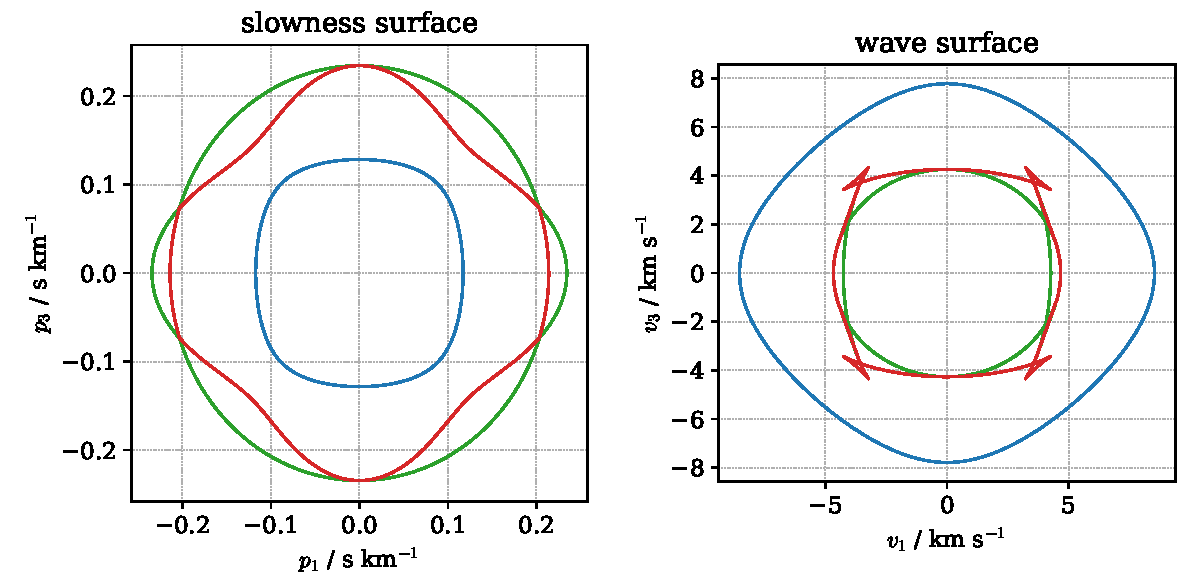
\includegraphics[width=0.95\textwidth]{figures/S1F1.pdf}
\caption{Sections through the slowness surface (left) and the wave surface (right) of a transversely isotropic medium, in the plane containing the symmetry axis; the sheets are coloured in order of speed. The quasi-P sheets are the innermost slowness curve and the outermost wave curve. The quasi-SV wave curve has cusps in directions where the corresponding slowness curve has inflection points.}
\label{fig:S1F1}
\end{figure}
\end{enumerate}

\end{document}